%%%%%%%%%%%%%%%%%%%%%%%%%%%%%%%%%%%%%%%%%%%%%%%%%%%%%%%%%%%%%%%%%%%%%%%%%%%%%%%%%%%%%%%%%%%%%%%
%                                          HYPEROPT                                           %
%%%%%%%%%%%%%%%%%%%%%%%%%%%%%%%%%%%%%%%%%%%%%%%%%%%%%%%%%%%%%%%%%%%%%%%%%%%%%%%%%%%%%%%%%%%%%%%
\chapter{Hyper-parameter Optimization of Neural Networks}
\label{chap:hyperopt}

\begin{chapabstract}
 Coucou
\end{chapabstract}

\minitoc

\newpage

%%%%%%%%%%%%%%%%%%%%%%%%%%%%%%%%%%%%%%%%%%%%%%%%%%%%%%%%%%%%%%%%%%%%%%%%%%%%%%%%%%%%%%%%%%%%%%%
\section{Defining the Problem}

Plan: split generic/deep learning or by class of methods ?

==The problem of hyper-parameter optimization appears when a model is governed by multiple hyper-parameters that are difficult to manually tune due to a lack of understanding in their effects. The problem gets worse when the hyper-parameters are not independent and it becomes necessary to tune them at the same time. The most intuitive solution is to try all possible combinations, but it grows exponentially with the number of hyper-parameters, making this approach usually unusable in practice.

==In practice, as it is usually impossible to prove the optimality of a solution without trying them all, the accepted solution is the best found in the budget allocated by the user to the search.

==Even though this problem appears in all kinds of situation, we are interested here in the optimization of deep learning models, as they have many hyper-parameters and we lack the understanding and the theoretical tools to tune them.

%%%%%%%%%%%%%%%%%%%%%%%%%%%%%%%%%%
\subsection{As Black-box Optimization}

==The hyper-parameter space $\mathcal{X}$ can be seen as a hypercube where each dimension is a hyper-parameter and each point $x$ of this space defines a unique model $f$. The performance of a model is given by a loss function $\mathcal{L}$. The goal of hyper-parameter optimization is to find the combination $x_*$ minimizing the loss function $\mathcal{L}$:
\begin{equation}
	x_* = \argmin_{x \in \mathcal{X}} \mathcal{L}(f(x))
\end{equation}

==The simplest method is random search. The idea is simply to pick combinations randomly from a uniform distribution. It is surprisingly efficient. This can be explained by the fact that all hyper-parameters are not equally relevant. In practice, only a few have a high impact on the loss~\cite{bergstra2012JMLR}. It is therefore likely to pick quickly a combination with optimal values for those hyper-parameters. Figure~\ref{fig:rs} shows this in a simple case. One of the dimensions clearly has more impact on the loss than the others, and random search allows us to find a better value of this parameter than grid search, for an equal number of tried combinations.

\begin{figure}[htb]
	\begin{minipage}[b]{.49\linewidth}
		\centering
		\centerline{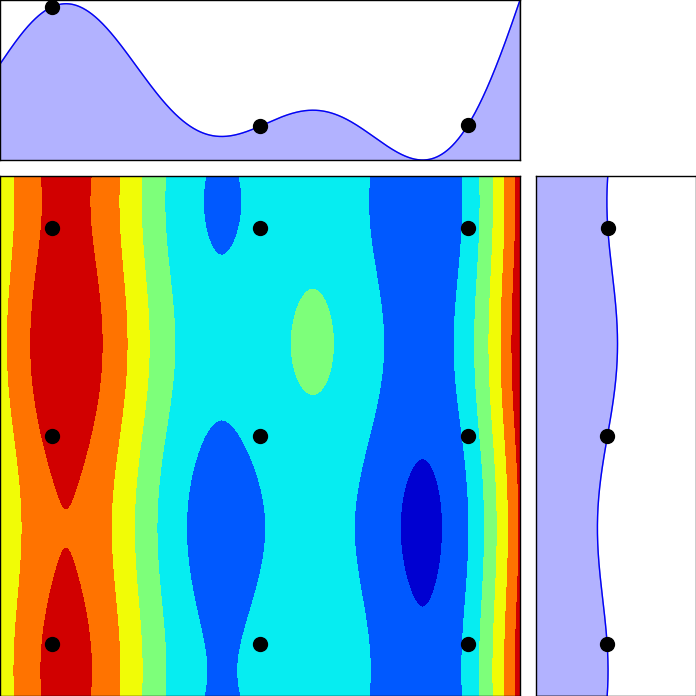
\includegraphics[width=7.2cm]{img_hyperopt/rs_grid}}
	\end{minipage}
	\begin{minipage}[b]{.49\linewidth}
		\centering
		\centerline{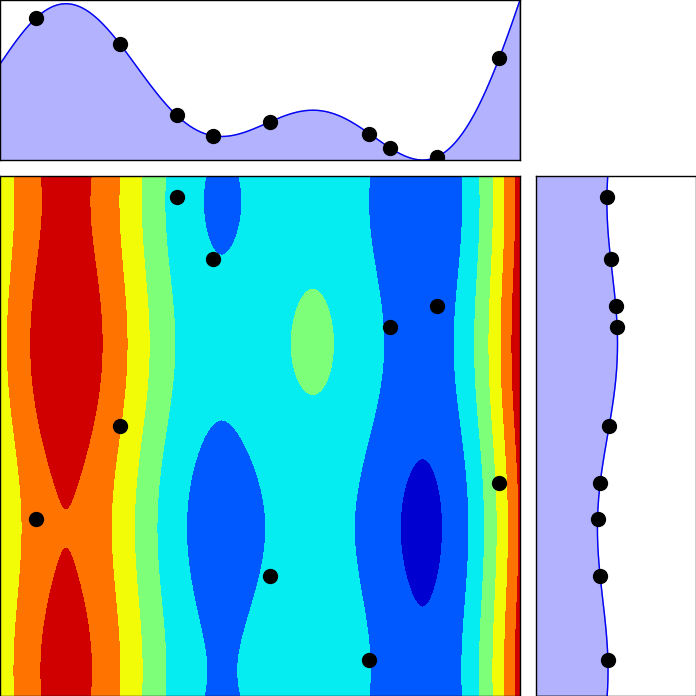
\includegraphics[width=7.2cm]{img_hyperopt/rs_random}}
	\end{minipage}
	\caption{Loss function for a two dimensional space. (Left) Grid search. (Right) Random search. At equal number of tried combinations, random search finds a better solution.}
	\label{fig:rs}
\end{figure}

==Can we do better than random search? Instead of picking combinations randomly from a uniform distribution, we could model the loss directly from the hyper-parameters, then pick the most promising configurations from this model. This is the idea behind Bayesian optimization, which we present in details in Section~\ref{sec:bo}.

==The task of building neural networks is well suited to the use of evolutionary algorithms. Networks can be split and combined in many ways due to their graph structure. It can be done at the layer level or even the unit level. Historically, NEAT~\cite{stanley2002EC} was the most efficient algorithm of this kind. More recent approaches such as~\cite{real2017ICML} or~\cite{miikkulainen2017} are able to explore extremely diverse and atypical network structures, while giving state-of-the-art results. They do require however a huge amount of computation.


As a black-box optimisation problem: random search, bayesian optimisation

Random Search~\textcite{bergstra2012JMLR}

GP + Tree of Parzen Estimator~\textcite{bergstra2011NIPS}

CMA-ES

%%%%%%%%%%%%%%%%%%%%%%%%%%%%%%%%%%
\subsection{As Meta-learning}

==Recently, reinforcement learning methods have been considered for this task~\cite{baker2017ICLR}~\cite{zoph2017ICLR}. A neural network called the controller is trained to build other neural networks, extremely efficient for a given task. It offers the possibility of transfer learning by reusing the controller on tasks similar to the initial one. The difficulty is in training the controller, which requires to build and train thousands of networks. 

==One major advantage of the last two approaches is the ability to use conditional hyper-parameters, i.e. hyper-parameters that must be chosen only if another hyper-parameter was chosen at a particular value. Bayesian Optimization one the one hand and Hyperband on the other hand have no simple way to integrate such hyper-parameters.

As a meta-learning problem: learning to learn, architecture learning

Large scale evolution

%%%%%%%%%%%%%%%%%%%%%%%%%%%%%%%%%%
\subsection{Other approaches}

==In the context of deep learning, the problem can be seen as a multi-armed bandit. The idea is to evaluate the models as soon as possible and discard the unpromising ones without wasting more time training them. The time gained can then be spent trying more models. Section~\ref{ssec:hyperband} describes an algorithm using this concept.

Bandit: Hyperband~\textcite{li2017ICLR}

Spectral Approach~\textcite{hazan2018ICLR}

Extrapolation of learning curves

%%%%%%%%%%%%%%%%%%%%%%%%%%%%%%%%%%
\subsection{Synthesis}

Can we unify all those approaches in the same framework ?

%%%%%%%%%%%%%%%%%%%%%%%%%%%%%%%%%%%%%%%%%%%%%%%%%%%%%%%%%%%%%%%%%%%%%%%%%%%%%%%%%%%%%%%%%%%%%%%
\section{Bayesian Optimization}
\label{sec:bo}

Bayesian Optimization is a method for optimizing the parameters of a black-box that is costly to evaluate. In deep learning the black-box is a neural network and the parameters are the hyper-parameters of the network. Evaluating it corresponds to training the network and computing the performance on the validation set. A recent and general review of the topic can be found in~\textcite{shahriari2016IEEE} where it is treated as an optimization method, while~\textcite{snoek2012NIPS} review the topic in the context of optimizing the hyper-parameters of machine learning models.

There are two components to Bayesian Optimization. First is a probabilistic model of the loss function, i.e. a function that takes the values of the hyper-parameters as input and estimate the value of the loss the corresponding neural network would have. Our model of choice is Gaussian processes which we present in Section~\ref{ssec:gp}. The second component, called the acquisition function, samples the model of the loss function to select the next set of hyper-parameters to evaluate. Common acquisition functions are presented in Section~\ref{ssec:acqfunc}.

%%%%%%%%%%%%%%%%%%%%%%%%%%%%%%%%%%
\subsection{Gaussian Processes}
\label{ssec:gp}

A Gaussian process is a supervised learning model mainly used for regression problems. It is a distribution over functions, i.e. from a set of data points, the Gaussian process gives us possible functions that fit those points, weighted by their likelihood. The shape and properties of possible functions are defined by a covariance function. When predicting the value of an unseen point, the Gaussian process returns a Normal distribution, with the variance an estimation of the uncertainty of the model at this point. Predicting multiple points will result in a joint Gaussian distribution.

Following the notation of~\textcite{rasmussen2005}, we write the Gaussian process as

\begin{equation}
    \mathrm{y}(\mathrm{x}) \sim \mathcal{GP} \left( m(\mathrm{x}), k(\mathrm{x}, \mathrm{x'}) \right)
\end{equation}

where $m(\mathrm{x})$ is the mean function which we set to $0$ for simplicity (in practice, just remove the mean of the predicted values from your dataset), and $k(\mathrm{x}, \mathrm{x'})$ is the covariance function which specifies the covariance between pair of data points. From this function we can build the covariance matrix of a set $\mathrm{X}$ of $N$ data points as

\begin{equation}
    K(\mathrm{X}, \mathrm{X}) = 
    \begin{pmatrix}
    k(\mathrm{x_1}, \mathrm{x_1}) & k(\mathrm{x_1}, \mathrm{x_2}) & \cdots & k(\mathrm{x_1}, \mathrm{x_N}) \\
    k(\mathrm{x_2}, \mathrm{x_1}) & k(\mathrm{x_2}, \mathrm{x_2}) & \cdots & k(\mathrm{x_2}, \mathrm{x_N}) \\
    \vdots & \vdots & \ddots & \vdots \\
    k(\mathrm{x_N}, \mathrm{x_1}) & k(\mathrm{x_N}, \mathrm{x_2}) & \cdots & k(\mathrm{x_N}, \mathrm{x_N})
    \end{pmatrix}
\end{equation}

This matrix is all we need to draw samples from the distribution. We pick a set $\mathrm{X_*}$ of points, build the covariance matrix $K(\mathrm{X_*}, \mathrm{X_*})$, then generate samples from this Gaussian distribution:

\begin{equation}
    \mathrm{y_*} \sim \mathcal{N} \left( 0, K(\mathrm{X_*}, \mathrm{X_*})\right)
\end{equation}

Some such samples are shown in Figure~\ref{fig:gp_prior}. The covariance function chosen for now is the squared exponential kernel:
\begin{equation}
	k(\mathrm{x}, \mathrm{x'}) = \sigma^2 \exp\left( -\frac{||\mathrm{x} - \mathrm{x'}||_2}{2l^2}\right)
\end{equation}
Other kernels and their properties are discussed later. 

Back to Figure~\ref{fig:gp_prior}, the thick blue line represents the mean of the distribution and the blue area around is the $95 \%$ prediction interval, i.e. all drawn samples will be in this interval with a probability of $95 \%$ (for a Normal distribution this is equal to $1.96 \sigma$). 

%The covariance matrix is a Gram matrix, meaning it is positive semi-definite, i.e. it admits a unique Cholesky decomposition

\begin{figure}[htb]
	\centering
	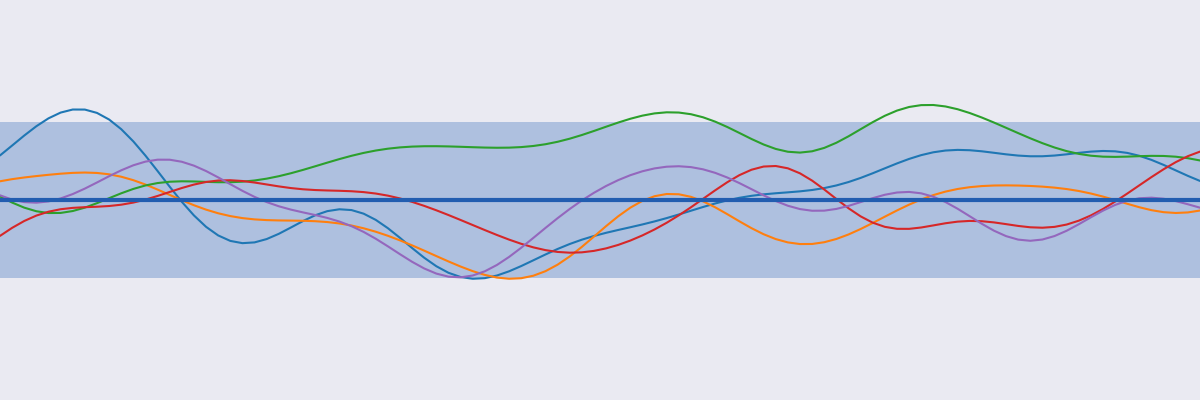
\includegraphics[width=\linewidth]{img_hyperopt/gp_prior.png}
	\caption{Gaussian process prior using a squared exponential kernel. The thin colored lines are samples drawn from the Gaussian process.}
	\label{fig:gp_prior}
\end{figure}

In probabilistic terms, this corresponds to the prior. Given a set of observed points $(\mathrm{X}, \mathrm{y})$ and a set of points we want to predict $(\mathrm{X_*}, \mathrm{y_*})$, the prior corresponds to $p\left( \mathrm{y_*} | \mathrm{X_*}, \theta \right)$ ($\theta$ are the hyper-parameters of the model which we will deal with later). We are interested in the posterior $p\left( \mathrm{y_*} | \mathrm{X_*}, \mathrm{X}, \mathrm{y}, \theta \right)$ i.e. the distribution of the new points conditioned on the points we have already observed. From probability theory we know that the posterior is

\begin{equation}
    p\left( \mathrm{y_*} | \mathrm{X_*}, \mathrm{X}, \mathrm{y}, \theta \right)
    =
    \frac{p\left( \mathrm{y}, \mathrm{y_*} | \mathrm{X}, \mathrm{X_*}, \theta \right)}{p\left( \mathrm{y} | \mathrm{X}, \theta \right)}
\end{equation}

The numerator is called the joint distribution and the denominator is the marginal likelihood. First, we compute the joint distribution

\begin{equation}
    \begin{bmatrix}
    \mathrm{y} \\
    \mathrm{y_*}
    \end{bmatrix}
    \sim
    \mathcal{N} \left( 0, 
    \begin{bmatrix}
    K(\mathrm{X}, \mathrm{X}) & K(\mathrm{X}, \mathrm{X_*}) \\
    K(\mathrm{X_*}, \mathrm{X}) & K(\mathrm{X_*}, \mathrm{X_*})
    \end{bmatrix}
    \right)
\end{equation}

Training a Gaussian process simply means pre-computing $K(\mathrm{X}, \mathrm{X})$, i.e. the covariance between the data points. At inference, we compute the covariance $K(\mathrm{X_*}, \mathrm{X_*})$ between the points we want to predict, and the covariance between the points we have observed and the points we want to predict $K(\mathrm{X}, \mathrm{X_*})$. And since the covariance matrix must be symmetrical, $K(\mathrm{X_*}, \mathrm{X}) = K(\mathrm{X}, \mathrm{X_*})^T$. For notational simplicity we will denote them $K$, $K_*$ or $K_*^T$ and $K_{**}$.

But the joint distribution isn't enough, it will generate functions that do not match the observed data. The posterior is obtained by conditioning the joint distribution to the observations, and because every term involved is a Gaussian distribution, there is a well-known result giving us the following equation

\begin{equation}
    p\left( \mathrm{y_*} | \mathrm{X_*}, \mathrm{X}, \mathrm{y}, \theta \right)
    =
    \mathcal{N} \left( K_* K^{-1} y, 
    K_{**} - K_* K^{-1} K_*^T \right)
\end{equation}

\begin{figure}[htb]
    \centering
    \begin{subfigure}[b]{\textwidth}
        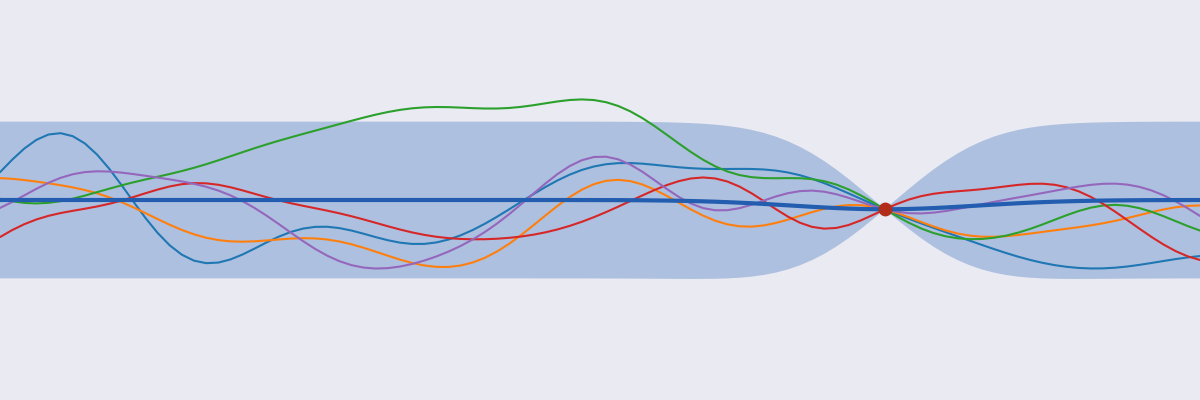
\includegraphics[width=\textwidth]{img_hyperopt/gp_posterior_1_point}
    \end{subfigure}

    \begin{subfigure}[b]{\textwidth}
        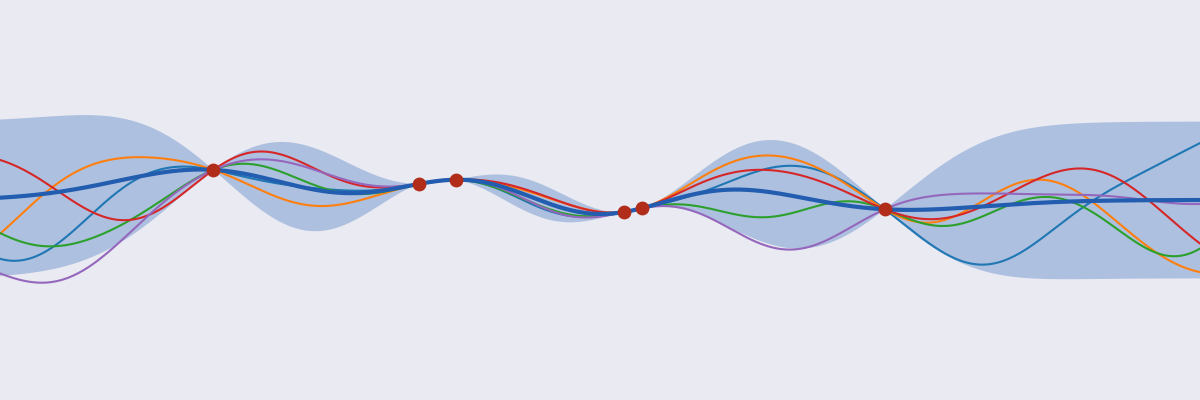
\includegraphics[width=\textwidth]{img_hyperopt/gp_posterior_6_point}
    \end{subfigure}
    \caption{Gaussian process posterior after fitting one point on top, six on the bottom. Notice how all the samples now go through those points and how the variance is lower close to them.}
    \label{fig:gp_posterior}
\end{figure}

Figure~\ref{fig:gp_posterior} shows what samples from this distribution looks like on a one dimensional problem. Each sample must go through every observed point, and the closer the points are, the less freedom the samples have to change. We also observe that outside of the range of points, the distribution quickly reverts to its prior. This is a property of this kernel, which is ill-suited for extrapolation.

So far we have assumed for simplification that the data is noise-free, however it is important to note that Gaussian processes are particularly well-adapted at dealing with noisy data. See~\textcite{rasmussen2005} for the changes to the equations.

We glossed over the choice of kernel until now. The most common is the one we used so far, the squared exponential kernel
\begin{equation}
	k(\mathrm{x}, \mathrm{x'}) = \sigma^2 \exp\left( -\frac{||\mathrm{x} - \mathrm{x'}||_2}{2l^2}\right)
\end{equation}

This kernel has two hyper-parameters $\theta = \{ \sigma^2 , l \}$. $\sigma^2$ controls the scale of the predicted output and $l$ is a vector of same dimensionality as $\mathrm{x}$ called the characteristic length-scale which measures how much a change along each dimension affects the output. A low value means that a small change in the input results in a big change in the output. 

The samples from this kernel are very smooth, and are in fact infinitely differentiable. This is usually too unrealistic for the process we are trying to model. In the context of Bayesian optimization, a more realistic alternative is the Matérn $5/2$ kernel
\begin{equation}
    k(r) = \sigma^2 \left( 1 + \frac{\sqrt{5}r}{l} + \frac{5r^2}{3l^2} \right) \exp \left( - \frac{\sqrt{5}r}{l}\right)
\end{equation}

where $r = \mathrm{x} - \mathrm{x'}$. The Matérn covariance functions are a class of kernel with two parameters $l$ and $\nu$. $\sigma^2$ and $l$ have the same role as for the squared exponential kernel and $\nu$ is a measure of how smooth the function is. The chosen value of $\nu = 5/2$ means the samples will be twice differentiable. $\nu = 1/2$ results in a very rough function while $\nu \to \infty$ is the squared exponential kernel. $5/2$ is a good compromise between too smooth and too difficult to optimize $\theta$ as many point estimate methods requires twice differentiability (\textcite{snoek2012NIPS}). Figure TODO shows what samples from these kernels look like.

[TODO fig influence of $\nu$]

The kernels presented have the common property of being stationary, i.e they depend only of $\mathrm{x} - \mathrm{x'}$. They are invariant to translation. It's very relevant in the context of hyper-parameter optimization as the kernels make no difference between values of 3 and 2 or 1000 and 999. Depending on the meaning of the hyper-parameters, this is not desirable. The solution is to use a non-stationary kernel, which we discuss in Section~\ref{ssec:nosta}.

Another problem of those kernels is that they have themselves hyper-parameters $\theta$ which needs to be chosen. As said before, $l$ is the characteristic length-scale. By construction of those covariance functions and as shown in~\textcite{neal1996phd}, the inverse of the length-scale determines how relevant an input is. In the context of hyper-parameter optimization, it can help us choose which hyper-parameters to tune carefully. It is therefore very important to select the correct value for $l$. 

There are two ways to learn $\theta$. The first is to maximize the marginal likelihood, which can be derived to  
\begin{equation}
	\log p\left(\mathrm{y} | \mathrm{X}, \theta \right) = - \frac{1}{2} \mathrm{y}^T K^{-1} \mathrm{y} - \frac{1}{2} \log |K| - \frac{n}{2} \log 2 \pi
\end{equation}

The optimization can be done with any off-the-shelf method, eventually with multiple restarts as there are no guarantee of a unique optima. 
%For example, the scikit-learn (\textcite{pedregosa2011sklearn}) implementation uses BFGS with 10 restarts by default.

The other solution is to not learn $\theta$ at all and instead marginalize the hyper-parameters, i.e. at inference compute 
\begin{equation}
    p\left( \mathrm{y_*} | \mathrm{X_*}, \mathrm{X}, \mathrm{y} \right)
    = \int p\left( \mathrm{y_*} | \mathrm{X_*}, \mathrm{X}, \mathrm{y}, \theta \right) p \left( \theta | \mathrm{X}, \mathrm{y} \right) d\theta
\end{equation}

This integral is usually intractable but can be approximated by sampling methods. \textcite{murray2010NIPS} use slice sampling, \textcite{garbuno2016CSDA} use asymptotically independent Markov sampling and \textcite{titsias2011} review different Monte Carlo methods used for this problem.

For a more extensive treatment on Gaussian Processes, see~\textcite{rasmussen2005}.

%%%%%%%%%%%%%%%%%%%%%%%%%%%%%%%%%%
\subsection{Acquisition Functions}
\label{ssec:acqfunc}

==Our chosen acquisition function is the Expected Improvement~\cite{jones2001}, which uses the improvement function $I$~\cite{shahriari2016IEEE}:
\begin{equation}
	I(x) = \left(y_* - \mu(x) \right) \mathds{1} \left(y_* > \mu(x) \right)
\end{equation}
where $x$ represents a given configuration, $y_*$ is the minimum loss found so far and $\mu$ is the mean returned by the Gaussian process. It will be $0$ if the predicted mean is less than the best loss found so far (which means that there is no improvement), otherwise it is proportional to the gap between the predicted mean and best loss. From there, the Expected Improvement is:
\begin{equation}
	EI(x) = \mathbb{E}[I(x)] = s(x) [u\Phi(u)+\phi(u)]
\end{equation}
with
\begin{equation}
	u = \frac{y_* - \mu(x)}{\sigma(x)}
\end{equation}
where $\sigma$ is the variance returned by the Gaussian process, and $\Phi$ and $\phi$ are the normal cumulative distribution and density function, respectively.

==This function offers a good compromise between exploration of regions with high uncertainty and exploitation. Moreover, it does not add any hyper-parameter to tune. Once we have computed EI for each configuration, we do not pick the argmax as classically done in the literature but we normalize the results to make a distribution from which we sample the next configurations to test.

Probability of Improvement

Expected Improvement

Upper Confidence Bound

Thompson Sampling

Entropy-search Portfolio

%%%%%%%%%%%%%%%%%%%%%%%%%%%%%%%%%%
\subsection{Tying it together}

\begin{figure}[htb]
	\centering
	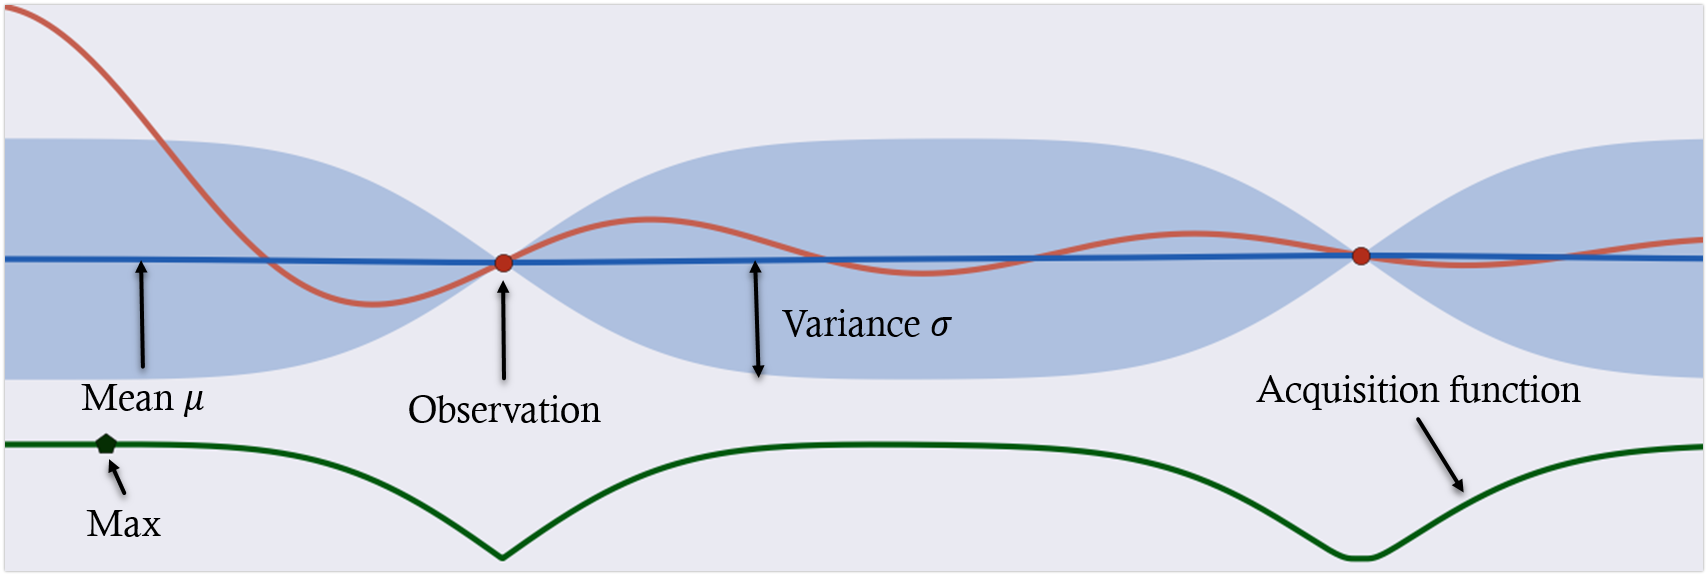
\includegraphics[width=\linewidth]{img_hyperopt/bo.png}
	\caption{Bayesian Optimization on a one dimensional function. The orange curve is the true loss function, the blue one is the prediction of the Gaussian process. The green curve is the acquisition function. The next evaluation will be at the maximum of the green curve.}
	\label{fig:bo}
\end{figure}

Hyperopt~\textcite{bergstra2013ICML}

Practical~\textcite{snoek2012NIPS}

%%%%%%%%%%%%%%%%%%%%%%%%%%%%%%%%%%
\subsection{Practical Challenges}

==One important aspect of this method is that the training time of the model is a dimension of the hyper-parameter space. This means that the method is free to choose how long to train each model. In practice we found that it prefers longer training time, even though it looks like a lower training time is enough to get a good estimate of the worth of the model and would allow the evaluation of more models. This is a flaw of the method, which lacks an explicit notion of budget and a way to best exploit it.

\subsubsection{Choosing kernel parameters}

Optimization, sampling

\subsubsection{Conditional spaces}

Tree of Parzen Estimator

Open problem using GP

\subsubsection{Parallelization}

Open problem using GP

See combination with Hyperband for a potential solution

\subsubsection{Non-stationarity}
\label{ssec:nosta}

Input Warping~\textcite{snoek2014ICML}

\subsubsection{Scaling}

Doesn't work well in high-dimension or with thousands of data points

Conditional neural processes ?

%%%%%%%%%%%%%%%%%%%%%%%%%%%%%%%%%%
\subsection{Contribution: Incremental Cholesky decomposition}

One of the big timesink of GP: computing the Cholesky decomposition. But in BO, the Gram matrix between calls is mostly the same, just with new rows. So we can store the decomposition and just update it.

==An important property of Gaussian processes is that the Gram matrix $K$ always has a unique Cholesky decomposition ($K$ is definite positive). This property is used in practice for the prediction of the mean and variance because it is necessary to invert $K$, and it is much more efficient to invert the Cholesky decomposition $L$.

==We use here the structure of the Gram matrix and a property of Bayesian optimization in order to reduce significantly the cost of the decomposition. The property is the following: at every call of the Gaussian process, our training set contains $n$ points from before and $k$ new points. By keeping the order of the points, the new Gram matrix is always structured as follows:
\begin{equation}
	K_{(n+k,n+k)} = 
    \begin{pmatrix}
    K_{(n,n)} & K_{(k,n)}^T \\
    K_{(k,n)} & K_{(k,k)}
  \end{pmatrix}
\end{equation}

==Moreover,
\begin{equation}
	 K_{(n,n)} = L_{(n)} L_{(n)}^T
\end{equation}
is already known. The question is then: can we compute $L_{(n+k)}$ from $L_{(n)}$ and the $k$ new points? The answer is positive, and after a bit of arithmetics omitted here, we get this:
\begin{equation}
  L_{(n+k)} = 
  \begin{pmatrix}
    L_{(n)} & 0 \\
    K_{(k,n)} (L_{(n)}^T)^{-1} & L_{(k)}
  \end{pmatrix}
\end{equation}

==It is also possible to get a formula for $ L_{(n+k)}^{-1}$:
\begin{equation}
  L_{(n+k)}^{-1} =
  \begin{pmatrix}
    L_{(n)}^{-1} & 0 \\
    - L_{(k)}^{-1} K_{(k,n)} (L_{(n)}^T)^{-1} L_{(n)}^{-1} & L_{(k)}^{-1}
  \end{pmatrix}
\end{equation}

==The complexity of the Cholesky decomposition is $O\left(\frac{(n+k)^3}{3}\right)$. In our case, this becomes $O\left(\frac{k^3}{3}\right)$ since it is still necessary to compute the decomposition of the $k$ new points.

%%%%%%%%%%%%%%%%%%%%%%%%%%%%%%%%%%%%%%%%%%%%%%%%%%%%%%%%%%%%%%%%%%%%%%%%%%%%%%%%%%%%%%%%%%%%%%%
\section{Application: Classification of MRI Field-of-View}

ISBI

%%%%%%%%%%%%%%%%%%%%%%%%%%%%%%%%%%
\subsection{Problem Description}

%%%%%%%%%%%%%%%%%%%%%%%%%%%%%%%%%%
\subsection{Baseline Results}

%%%%%%%%%%%%%%%%%%%%%%%%%%%%%%%%%%
\subsection{Hyper-parameter Optimization}

\begin{figure}[htb]
	\centering
	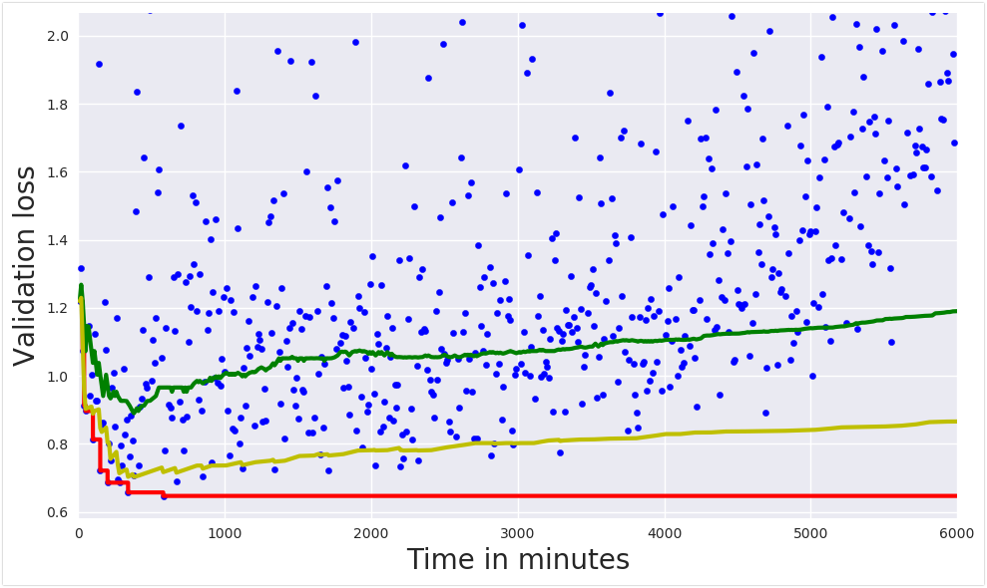
\includegraphics[width=.95\linewidth]{img_hyperopt/bo_acc_time.png}
	\label{fig:bo_acc_time}
\end{figure}

\begin{figure}[htb]
	\centering
	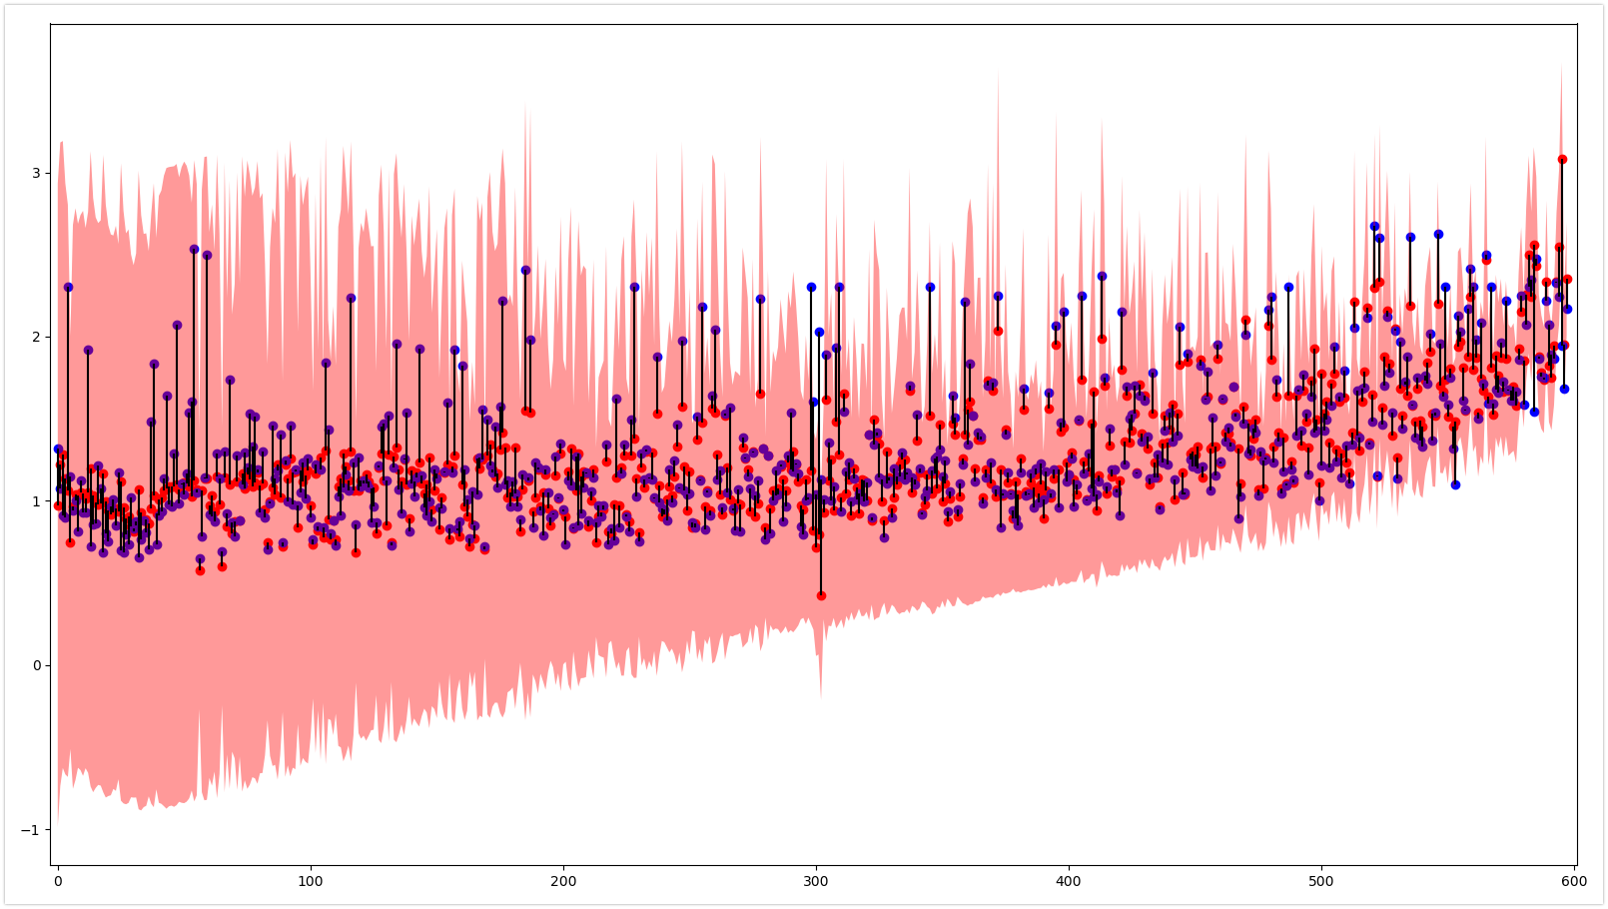
\includegraphics[width=.95\linewidth]{img_hyperopt/bo_error_time.png}
	\label{fig:bo_error_time}
\end{figure}

%%%%%%%%%%%%%%%%%%%%%%%%%%%%%%%%%%%%%%%%%%%%%%%%%%%%%%%%%%%%%%%%%%%%%%%%%%%%%%%%%%%%%%%%%%%%%%%
\section{Contribution: Combining Bayesian Optimization and Hyperband}

CAp

%%%%%%%%%%%%%%%%%%%%%%%%%%%%%%%%%%
\subsection{Hyperband}
\label{ssec:hyperband}

==A property of neural networks is that their training is iterative, usually some variant of gradient descent. A consequence is that it is possible to interrupt training any time, evaluate the network, then resume training. This is the property Hyperband~\cite{li2017ICLR} takes advantage of.

==The principle is simple: pick randomly a group of configurations from a uniform distribution, train the corresponding networks partially, evaluate them, resume training of the most performing ones, and so on until a handful of them have been trained to completion. Then pick a new group and repeat the cycle until exhaustion of the available resources.

==But a problem appears: at which point in the training can we start evaluating the models? Too soon and they will not have started to converge, making the evaluation meaningless, too late and we have wasted precious resource training under-performing models. Moreover, we do not know how to find that point and it changes between tasks. Hyperband's answer is to divide a cycle into brackets. Each bracket has the same quantity of resource at its disposal. The difference between brackets is the point at which they start evaluating the models. The first bracket will start evaluating and discarding models very early, allowing it to try a bigger number of configurations, while the last bracket will try only a small number of configurations but will train them until the end.

==The algorithm is controlled by two hyper-parameters: the maximal quantity of resources $R$ that can be allocated to a given model, and the proportion of configurations $\eta$ kept at each evaluation. We chose $R = 27$ minutes and $\eta = 3$, which means that we keep $1/3$ of models at each evaluation.

%%%%%%%%%%%%%%%%%%%%%%%%%%%%%%%%%%
\subsection{Combining the methods}

%%%%%%%%%%%%%%%%%%%%%%%%%%%%%%%%%%
\subsection{Experiments on CIFAR-10}

%%%%%%%%%%%%%%%%%%%%%%%%%%%%%%%%%%%%%%%%%%%%%%%%%%%%%%%%%%%%%%%%%%%%%%%%%%%%%%%%%%%%%%%%%%%%%%%
\section{Conclusion}

When to optimize and with which method ?
